%%%%%%%%%%%%%%%%%%%%%%%%%%%%%%%%%%%%%%%%
% "ModernCV" CV and Cover Letter
% LaTeX Template
% Version 1.11 (19/6/14)
%
% This template has been downloaded from:
% http://www.LaTeXTemplates.com
%
% Original author:
% Xavier Danaux (xdanaux@gmail.com)
%
% License:
% CC BY-NC-SA 3.0 (http://creativecommons.org/licenses/by-nc-sa/3.0/)
%
% Important note:
% This template requires the moderncv.cls and .sty files to be in the same 
% directory as this .tex file. These files provide the resume style and themes 
% used for structuring the document.
%
%%%%%%%%%%%%%%%%%%%%%%%%%%%%%%%%%%%%%%%%%

%----------------------------------------------------------------------------------------
%	PACKAGES AND OTHER DOCUMENT CONFIGURATIONS
%----------------------------------------------------------------------------------------

\documentclass[11pt,a4paper,sans]{moderncv} % Font sizes: 10, 11, or 12; paper sizes: a4paper, letterpaper, a5paper, legalpaper, executivepaper or landscape; font families: sans or roman

\moderncvstyle{casual} % CV theme - options include: 'casual' (default), 'classic', 'oldstyle' and 'banking'
\moderncvcolor{blue} % CV color - options include: 'blue' (default), 'orange', 'green', 'red', 'purple', 'grey' and 'black'

\usepackage{lipsum} % Used for inserting dummy 'Lorem ipsum' text into the template
\usepackage[utf8]{inputenc}
\usepackage[scale=0.80]{geometry} % Reduce document margins
\usepackage{fontawesome}
\usepackage{fancyhdr}
\usepackage{ragged2e}
\usepackage{xcolor}

% Stuff for bibliography
\usepackage{mhchem}
\usepackage{natbib}
\renewcommand{\bibsection}{}

\def\changemargin#1#2{\list{}{\rightmargin#2\leftmargin#1}\item[]}
\let\endchangemargin=\endlist 

%\setlength{\hintscolumnwidth}{3cm} % Uncomment to change the width of the dates column
%\setlength{\makecvtitlenamewidth}{10cm} % For the 'classic' style, uncomment to adjust the width of the space allocated to your name
\definecolor{unazul}{HTML}{539bd7}
\newcommand*{\scholarsocialsymbol}{
\includegraphics[height=.7\baselineskip]{google-scholar}}
\newcommand*{\rgatesocialsymbol}{
\includegraphics[height=.75\baselineskip]{rgate}}
\newcommand*{\stackovsocialsymbol}{
\includegraphics[height=.75\baselineskip]{stacko}}

\makeatletter
\renewcommand*{\makeletterclosing}{
  \@closing\\[3em]%
  
\includegraphics[scale=.8]{pictures/signaturepanades.png}\\% Insert signature
  {Ramón L. Panad\'es-Barrueta}%
  \ifthenelse{\isundefined{\@enclosure}}{}{%
    \\%
    \vfill%
    {\color{color2}\itshape\enclname: \@enclosure}}}
\makeatother

%----------------------------------------------------------------------------------------
%	NAME AND CONTACT INFORMATION SECTION
%----------------------------------------------------------------------------------------

\firstname{\LARGE Ramón Lorenzo} % Your first name
\familyname{\Huge Panad\'es Barrueta} % Your last name

% All information in this block is optional, comment out any lines you don't need
\title{\href{https://panadestein.github.io}{panadestein.github.io}}
%  \title{\small Ave Paul Langevin, Residence REEFLEX A316, Villeneuve d'Ascq, France}
%\address{Residence REEFLEX B\^at. A-316}{Ave Paul Langevin, Cité Scientifique, 59650 VILLENEUVE D'ASCQ}
%\mobile{(+33) 769205894}
%\phone{(000) 111 1112}
%\fax{(000) 111 1113}
\social[github][github.com/Panadestein]{GitHub} 
\social[linkedin][www.linkedin.com/in/ram\%C3\%B3n-l-panad\%C3\%A9s-barrueta-phd-a3b851129/]{LinkedIn}
\collectionadd[rgate]{socials}{\href{https://www.researchgate.net/profile/Ramon_Panades-Barrueta}{ ResearchGate}}
\collectionadd[scholar]{socials}{\href{https://scholar.google.com/citations?user=IMWuq6wAAAAJ&hl=en}{ Google Scholar}}
\collectionadd[stackov]{socials}{\href{https://stackoverflow.com/users/5661001/panadestein?tab=profile}{ Stackoverflow}}
%\email{rpana92@gmail.com}
\homepage{panadestein.github.io} 
%\extrainfo{additional information}
\photo[75pt][0.3pt]{pictures/newlook_test_smaller.jpg} % The first bracket is the picture height, the second is the thickness of the frame around the picture (0pt for no frame)
%\quote{"A witty and playful quotation" - John Smith}

%----------------------------------------------------------------------------------------

\begin{document}

\makecvtitle % Print the CV title

%----------------------------------------------------------------------------------------
%	EDUCATION SECTION
%----------------------------------------------------------------------------------------

\vspace{6.0cm}

\section{Professional experience}

\cventry{Present\\01.08.2021}{Postdoctoral fellow}{\href{https://tu-dresden.de/}{\textcolor{unazul}{TU Dresden}}, Large-Scale Theoretical Spectroscopy group  (\href{https://golzegroup.org/}{\textcolor{unazul}{LSTS}})}{Germany}{}{}
\cvitem{}{Project:  Accurate, Exascale-Ready Methods for Theoretical Core-Level Spectroscopy of Complex Materials (\href{https://gepris.dfg.de/gepris/projekt/453275048?language=en}{\textcolor{unazul}{CoreXL}}). Dr. Dorothea Golze's Emmy-Noether group.}
\cvitem{}{This project aims at developing High-Performance theoretical methods for core-level spectroscopy, that will greatly benefit from the new generation of exascale supercomputers. The focus of my research in the group is the development of low-scaling GW-based algorithms for the prediction of XPS and XAS spectra. The former are implemented in the FHI-aims software package. Additional stand-alone libraries will be also developed in the framework of the \href{https://www.nomad-coe.eu/}{\textcolor{unazul}{NOMAD}} CoE.}

\cventry{31.07.2021\\01.11.2020}{Postdoctoral fellow}{\href{https://www.utwente.nl/en}{\textcolor{unazul}{University of Twente}}, Computational Chemical Physics Group  (\href{https://www.utwente.nl/en/tnw/ccp/}{\textcolor{unazul}{CCP}})}{Netherlands}{}{}
\cvitem{}{Project: Targeting Real chemical accuracy at the EXascale (\href{https://trex-coe.eu/}{\textcolor{unazul}{TREX}}). European HPC Centre of Excellence (\href{https://www.hpccoe.eu/index.php/trex-coe/}{\textcolor{unazul}{CoE}})}
\cvitem{}{This European CoE aims at developing open-source high-performance quantum chemistry software tailored to the emerging exascale architectures. As a member of Prof. Claudia Filippi's group, I contributed to the Cornell-Holland Ab-initio Materials Package (CHAMP). During my time in the project, I have employed innovative programming techniques like the Implicit Reference to Parameters method (IRP).}

\section{Education}

\cventry{23.10.2020 \\ 01.10.2017}{PhD in Physics}{\href{www.univ-lille.fr}{\textcolor{unazul}{University of Lille}}, Laboratoire de Physique des Lasers, Atomes et Molécules (\href{phlam.univ-lille.fr}{\textcolor{unazul}{PhLAM}})}{France}{}{}
\cvitem{}{Thesis title: Full quantum simulations of the interaction between atmospheric molecules and model soot particles (available at \href{https://theses.fr/2020LILUR022}{\textcolor{unazul}{theses.fr}})}
\cvitem{}{Supervisor: Prof. Dr. Daniel Pel\'aez-Ruiz (\href{http://www.ismo.u-psud.fr/spip.php?rubrique28&lang=fr}{\textcolor{unazul}{ISMO}}, Université Paris-Saclay)}

\cvitem{}{The subject of my thesis was the development and application of optimization and tensor decomposition algorithms for representing Potential Energy Surfaces. The later were employed in Nuclear Quantum Dynamics calculations with the Multiconfiguration Time-dependent Hartree (MCTDH) method.}

\cventry{23.06.2017\\12.09.2016}{MSc in Physics (International Master 2 Atmospheric Environments)}{\href{www.univ-lille.fr}{\textcolor{unazul}{University of Lille}}, Laboratoire de Physique des Lasers, Atomes et Molécules (\href{phlam.univ-lille.fr}{\textcolor{unazul}{PhLAM}})}{France}{}{}
%{\textbf{Distinction: \textit{Mention Bien}}}
\cvitem{}{Thesis title: Towards a quantum dynamical description of the photodissociation of $Cl_{2}$ molecule adsorbed on ice}
\cvitem{}{Supervisors: Prof. Dr. Daniel Pel\'aez-Ruiz and Prof. Dr. Maurice Monnerville}

\cventry{01.07.2016\\01.09.2011}{BSc in Radiochemistry}{\href{www.uh.cu}{\textcolor{unazul}{University of Havana}}, Higher Institute of Technologies and Applied Sciences (\href{www.instec.cu}{\textcolor{unazul}{InSTEC}})}{Havana, Cuba}{}{}
%{\textbf{Distinction: \textit{Summa Cum Laude}}}
\cvitem{}{Thesis title: Mean Potential Phase Space Theory study of the 
$Si({}^{3}P) + OH(X^{2}\Pi) \rightarrow SiO(X^{1}\Sigma^{+}) + H({}^{2}S)$ reaction}
\cvitem{}{Supervisor: Assoc. Prof. Dr. Alejandro Rivero-Santamar\'ia (\href{phlam.univ-lille.fr}{\textcolor{unazul}{PhLAM}}, Université de Lille)}

\section{Publications}

\cvitem{2021}{Panadés-Barrueta, R. L., Shepard , S. and Filippi, C. \textbf{State specific optimization of double excitations in quantum Monte Carlo}, \textcolor{unazul}{In preparation.}}
\cvitem{2020}{Panadés-Barrueta, R. L. and Peláez, D. (2020). \textbf{Low-Rank Sum-of-Products Finite-Basis-Representation (SOP-FBR) of Potential Energy Surfaces}, \href{https://doi.org/10.1063/5.0027143}{\textcolor{unazul}{Journal of Chemical Physics, \textbf{153}, 234110.}}}
\cvitem{2019}{Panadés-Barrueta, R. L., Martínez-Núñez, E., \& Peláez, D. (2019). \textbf{Specific Reaction Parameter Multigrid POTFIT (SRP-MGPF): Automatic Generation of Sum-of-Products Form Potential Energy Surfaces for Quantum Dynamical Calculations}, \href{https://doi.org/10.3389/fchem.2019.00576}{\textcolor{unazul}{Frontiers in Chemistry, \textbf{7}, 576.}} Included in the book \href{https://www.frontiersin.org/research-topics/9088/application-of-optimization-algorithms-in-chemistry}{\textcolor{unazul}{Application of Optimization Algorithms in Chemistry}}}
\cvitem{2016}{Panad\'es-Barrueta, R. L., Rubayo-Soneira, J., Monnerville, M., Larregaray, P., Dayou, F., and Rivero-Santamar\'ia, A. (2016). \textbf{Mean Potential Phase Space Theory study of the $\mathbf{Si({}^{3}P) + OH(X^{2}\Pi) \rightarrow SiO(X^{1}\Sigma^{+}) + H({}^{2}S)}$ reaction}, \href{http://www.revistacubanadefisica.org/index.php/rcf/article/view/65}{\textcolor{unazul}{Revista Cubana de Física, \textbf{33(2)}, 102-117.}}}


\section{Seminars and conferences}

\cventry{December 2021}{An overview of GW and its applications to core level spectroscopy}{}{}{}{\href{https://panadestein.github.io/gw_talk/sem_rpanades.html}{\textcolor{unazul}{Group seminar}} \\ TU Dresden, Germany}

\cventry{November 2020}{A \textit{gentle} introduction to MCTDH}{}{}{}{\href{https://nbviewer.org/github/Panadestein/mctdh_talk/blob/main/mctdh_intro.pdf}{\textcolor{unazul}{Group seminar}} \\ University of Twente, Netherlands}

\cventry{August 2020}{On the automatic computation of global (intermolecular) potential energy surfaces for quantum dynamical simulations}{Invited Speaker}{}{}{\href{http://spig2020.ipb.ac.rs/invited.html}{\textcolor{unazul}{Symposium and Summer School on Physics of Ionized Gases}} \\ Šabac, Serbia}
\cventry{February 2020}{Automatic computation of global (intermolecular) potential energy surfaces for
 (non) covalently bound systems}{Contributed Talk}{}{}{\href{https://jctmsifn.sciencesconf.org/program/details}{\textcolor{unazul}{Journée Chimie Théorique et Simulation Moléculaire IdF/Nord}} \\ Chimie ParisTech. Paris, France}
\cventry{April 2019}{Automatic computation of potential energy surfaces for covalently bound systems}{Seminar}{}{}{Laboratoire de Chimie Physique - Matière et Rayonnement (LCPMR). Paris, France}

%\newgeometry{top=1.5cm}
\section{Teaching experience}

\cventry{2021}{Qualification for a position as an assistant professor in a French University}{}{}{}{\textbf{Sections:} 30 and 31 of the \href{https://www.conseil-national-des-universites.fr/cnu/}{\textcolor{unazul}{CNU}} \space\space\space  \textbf{Qualification Numbers:} 21230359242 and 21231359242}
\cventry{2018--2019}{Laboratory of Thermodynamics}{}{}{}{\textbf{Place:} IUT A de Lille (University of Lille), France \space\space\space   \textbf{No. hours:} 64 \space\space\space  \textbf{Language:} French}
\cventry{2013--2016}{Mathematical Analysis and Linear Algebra}{}{}{}{\textbf{Place:} InSTEC (University of Havana), Cuba \space\space\space  \textbf{No. hours:} 72 \space\space\space  \textbf{Language:} Spanish}

\section{Reviewing activities}
\cvitem{}{List of Journals I have contributed as a reviewer.}
\cventry{2022}{Physical Review B}{}{(\href{https://journals.aps.org/prb/}{\textcolor{unazul}{PRB}})}{}{}


\section{Honors and Awards}

\cvitem{2019}{\textbf{Best Poster Prize} 10\textsuperscript{th} International Meeting on Atomic and Molecular Physics and Chemistry (IMAMPC). Madrid, Spain.}
\cvitem{2018}{\textbf{Best Poster Prize} 6\textsuperscript{th} High Dimensional Quantum Dynamics Workshop (HDQD). Lille, France.}
\cvitem{2018}{\textbf{PCCP Best Poster Prize} 9\textsuperscript{th} International Meeting on Atomic and Molecular Physics and Chemistry (\href{https://phlam.univ-lille.fr/detail-actu/ramon-panades-barrueta-le-prix-poster-du-journal-pccp-du-congres-imampc/}{\textcolor{unazul}{IMAMPC}}). Berlin, Germany.}
\cvitem{2015}{\textbf{ICPC Contestant} Caribbean Finals of the International Collegiate Programming Contest (ACM-ICPC). Havana, Cuba}
\cvitem{2010}{\textbf{IChO Contestant} Captain of the Cuba Team in the 42\textsuperscript{nd} International Chemistry Olympiad (\href{https://www.icho2010.org/en/results.html}{\textcolor{unazul}{IChO 2010}}). Tokyo, Japan}

%\clearpage

\section{Competitive research grants and fellowships}

\cventry{Oct.-Dec. 2019}{Research Grant German Academic Exchange Service (DAAD)}{}{}{}{Awarded by: Deutscher Akademischer Austausch Dienst \\ Place: Universität Heidelberg, \href{https://www.pci.uni-heidelberg.de/cms/index.html}{\textcolor{unazul}{Theoretical Chemistry Group}} \\ Supervisor: Prof. Dr. Oriol VENDRELL}
\cventry{2016--2017}{Labex CaPPA Fellowship}{}{}{}{Awarded by: Laboratoire d'excellence \href{http://www.labex-cappa.fr/master-atmospheric-environment/fellowships}{\textcolor{unazul}{CaPPA}} \\ Place: University of Lille }

\clearpage

\section{Research training and attended workshops}

\cventry{June 2022}{NOMAD WP2 Hackathon}{Academic Centre of the University of Latvia. Riga, Latvia}{}{}{}
\cventry{July 2021}{Stochastic Methods in Electronic Structure Theory}{Telluride Science Research Center (Virtual Workshop)}{}{}{}
\cventry{January 2020}{First general assembly of the GDR NBODY: N-body quantum problem in chemistry and physics}{Universit\'e de Lille, France}{}{}{}
\cventry{August 2019}{School EMIE-UP. Multiscale Dynamics in Molecular Systems}{École de Physique des Houches. Haute-Savoie, France}{}{}{}
\cventry{June 2019}{3\textsuperscript{rd} Mini-school on mathematics for theoretical chemistry and physics}{Sorbonne Université, Pierre et Marie Curie. Paris, France}{}{}{}
\cventry{June 2018}{Bridging experiment and theory in precision spectroscopy (BETS) 4\textsuperscript{th} MOLIM Training School}{Nicolaus Copernicus University. Torun, Poland}{}{}{}
\cventry{January 2018}{Label of Theoretical Chemistry \^Ile de France-Nord}{Sorbonne Universit\'e, Pierre et Marie Curie. Paris, France}{}{}{}
\cventry{October 2017}{Quantum Dynamics with the Multi-Configuration Time-Dependent Hartree (MCTDH) method: future and perspectives}{Universit\'e Paris-Saclay. Paris, France}{}{}{}
\cventry{March 2017}{International Conference on Aerosol Cycle (ICAC)}{Universit\'e de Lille, France}{}{}{}

%\section{Scientific skills}
%
%\cventry{2016--present}{Electronic Structure and Nuclear Quantum Dynamics}{\textit{Universit\'e  de Lille}}{France}{}{Acquired Computational Chemistry skills and performed development of methodologies, mainly applied to systems with atmospheric and astrophysical interest}
%\cventry{2011--Present}{GNU/Linux systems}{}{}{}{Involvement in the GNU/Linux community as a part of the professional work, in particular with the Arch Linux distribution}

\section{Computer skills}

%\faicon{github}
\cvitem{OS}{(\href{https://github.com/Panadestein/nixos-config.git}{\textcolor{unazul}{NixOS}}) Linux, UNIX}
\cvitem{Languages}{Fortran and C (HPC optimization and parallelization with ScaLAPACK), Python (scientific computing libraries), Julia, Wolfram Language, Bash, Lisp, \LaTeX, HTML/CSS}
\cvitem{Software}{\href{https://fhi-aims.org/}{\textcolor{unazul}{FHI-aims}} (low-scaling massively parallel GW algorithms), \href{https://www.pci.uni-heidelberg.de/tc/usr/mctdh/ref.html}{\textcolor{unazul}{MCTDH}} (Developed the SOP-FBR and SRPTucker packages), \href{https://www.utwente.nl/en/tnw/ccp/research/CHAMP.html}{\textcolor{unazul}{CHAMP}} (massively parallel QMC algorithms), \href{https://rxnkin.usc.es/index.php/AutoMeKin}{\textcolor{unazul}{AutoMeKin}}, MOPAC, Quantum package, MOLPRO, MOLCAS, Gaussian, Wolfram Mathematica, \href{https://panadestein.github.io/emacsd/}{\textcolor{unazul}{Emacs}}, Git, Inkscape, Libreoffice}
\cvitem{Numerical methods}{Tensor decomposition, Optimization Algorithms, Quantum Monte Carlo, low-scaling GW algorithms}


\section{Languages (CEFR)}

%\begin{minipage}{.5\textwidth}
\cvitemwithcomment{Spanish}{Native speaker}{}
%\end{minipage}% This must go next to `\end{minipage}`
%\begin{minipage}{.5\textwidth}
\cvitemwithcomment{English}{Proficient user (C1)}{}
%\end{minipage}
%\begin{minipage}{.5\textwidth}
\cvitemwithcomment{French}{Proficient user (C1)}{}
%\end{minipage}% This must go next to `\end{minipage}`
%\begin{minipage}{.5\textwidth}
\cvitemwithcomment{German}{Basic user (A2, Goethe-Institut certified)}{}
%\end{minipage}

%----------------------------------------------------------------------------------------
%	INTERESTS SECTION
%----------------------------------------------------------------------------------------

%\section{Interests}
%
%\renewcommand{\listitemsymbol}{-~} % Changes the symbol used for lists
%
%\cvlistdoubleitem{Physical-Chemistry}{Mathematics}
%\cvlistdoubleitem{Programming}{Free Software}
%\cvlistdoubleitem{Theoretical research}{Music}

%----------------------------------------------------------------------------------------
%	COVER LETTER
%----------------------------------------------------------------------------------------

% To remove the cover letter, comment out this entire block

%\clearpage
%\thispagestyle{empty}
%
%\recipient{Consulaat-generaal van de\\ Bondsrepubliek Duitsland te Amsterdam}{Honthorststraat 36-38\\1071 DG Amsterdam, Nederland} % Letter recipient
%\date{June 7, 2021} % Letter date
%\opening{Dear Sir or Madam,} % Opening greeting
%\closing{Sincerely yours,} % Closing phrase
%%\enclosure[Attached]{Certificates} % List of enclosed documents
%
%\makelettertitle{} % Print letter title
%\justify{}
%My name is Ramón Lorenzo Panadés Barrueta.  I am hereby applying for the EU Blue Card in Germany. Starting from August 1st, 2021, I will be employed as a postdoctoral researcher at TU Dresden. The expertise that I have acquired during my Master’s and Ph.D. at the University of Lille, France, as well as my time as a postdoctoral researcher at the University of Twente, Netherlands, lies in the fields of Theoretical and Computational Chemistry, High-Performance Computing (HPC) and Research Software Engineering. These skills are in high demand in the German labor market. For further details on my background and qualifications, please refer to the attached CV\@.
%
%In addition to my professional occupation in Germany, I also have personal reasons to apply for a Blue Card. My fiancee is German, and we plan to relocate together to Dresden. To facilitate my integration, I have been studying the German language in the past months. Please find attached to this letter a certificate of participation in an A2.2 course certified by the Goethe Institut. 
%
%Considering my expertise in a highly demanded field which makes me a valuable asset for the German labor market, and my relation to Germany, I hope you will provide me with the EU Blue Card.
%
%\makeletterclosing{} % Print letter signature

%----------------------------------------------------------------------------------------
%	References
% ----------------------------------------------------------------------------------------

%\clearpage
%
%\thispagestyle{empty}
%\begin{center}
%\LARGE \textbf{References}
%\end{center}
%\vspace{3cm}
%
%\begin{itemize}
%\item \textbf{Prof. Dr. Daniel Peláez}\\
% \vspace{-.5cm}
% \begin{changemargin}{}{} 
%  Institut des Sciences Moléculaires d’Orsay (ISMO)\\
%  UMR 8214, Bât. 520, Université Paris-Saclay\\
%  91405 Orsay Cedex, France \\
%  \textbf{Phone:} +33 6 28 78 79 51\\
%  \textbf{Email:} daniel.pelaez-ruiz@universite-paris-saclay.fr
% \end{changemargin}
%  
% \vspace{2cm}
% 
%\item \textbf{Prof. Dr. Oriol Vendrell}\\
% \vspace{-.5cm}
% \begin{changemargin}{}{} 
%  Chair of Theoretical Chemistry, Universität Heidelberg\\
%  Im Neuenheimer Feld 229\\
%  69120 Heidelberg, Germany\\
%  \textbf{Phone:} +49 6221/54 52 15\\
%  \textbf{Email:} oriol.vendrell@uni-heidelberg.de
% \end{changemargin}
%\end{itemize}

%----------------------------------------------------------------------------------------
%	Abstract
% ----------------------------------------------------------------------------------------

%\clearpage
%
%\begin{center}
%\textbf{Abstract of the Doctoral Dissertation}
%\end{center}
%
%My PhD aims at simulating full quantum mechanically (nuclei and electrons) the processes of adsorption and photoreactivity of NO\(_2\) adsorbed on soot particles (modeled as large Polycyclic Aromatic Hydrocarbons, PAHs) in atmospheric conditions. A detailed description of these processes is necessary to understand the differential day-nighttime behavior of the production of HONO~\cite{guan2017identification,monge2010light}, which is a precursor of the hydroxyl radical (OH)~\cite{holloway2015atmospheric}. In particular, the specific mechanism of the soot-mediated interconversion between NO\(_2\) and HONO is to date not fully understood. Due to  its particular relevance in this context, we have chosen the Pyrene-NO\(_2\) as our model system~\cite{guan2017identification}.\\
%
%The first stage in this study has consisted of the determination of the stable configurations (transition states and minima) of the Pyrene-NO\(_2\) system. To this end, we have used the recently developed van der Waals Transition State Search using Chemical Dynamics Simulations (vdW-TSSCDS) method~\cite{kopec2019vdw}, the generalization of the TSSCDS algorithm developed in our group. In this way, the present work represents the first application of vdW-TSSCDS to a large system (81D)~\cite{panades2021}. Starting from a set of judiciously chosen input geometries, the aforementioned method permits the characterization of the topography of an intermolecular Potential Energy Surface (PES), or in other words the determination of the most stable conformations of the system, in a fully automated and efficient manner. \\
%
%\begin{center}
%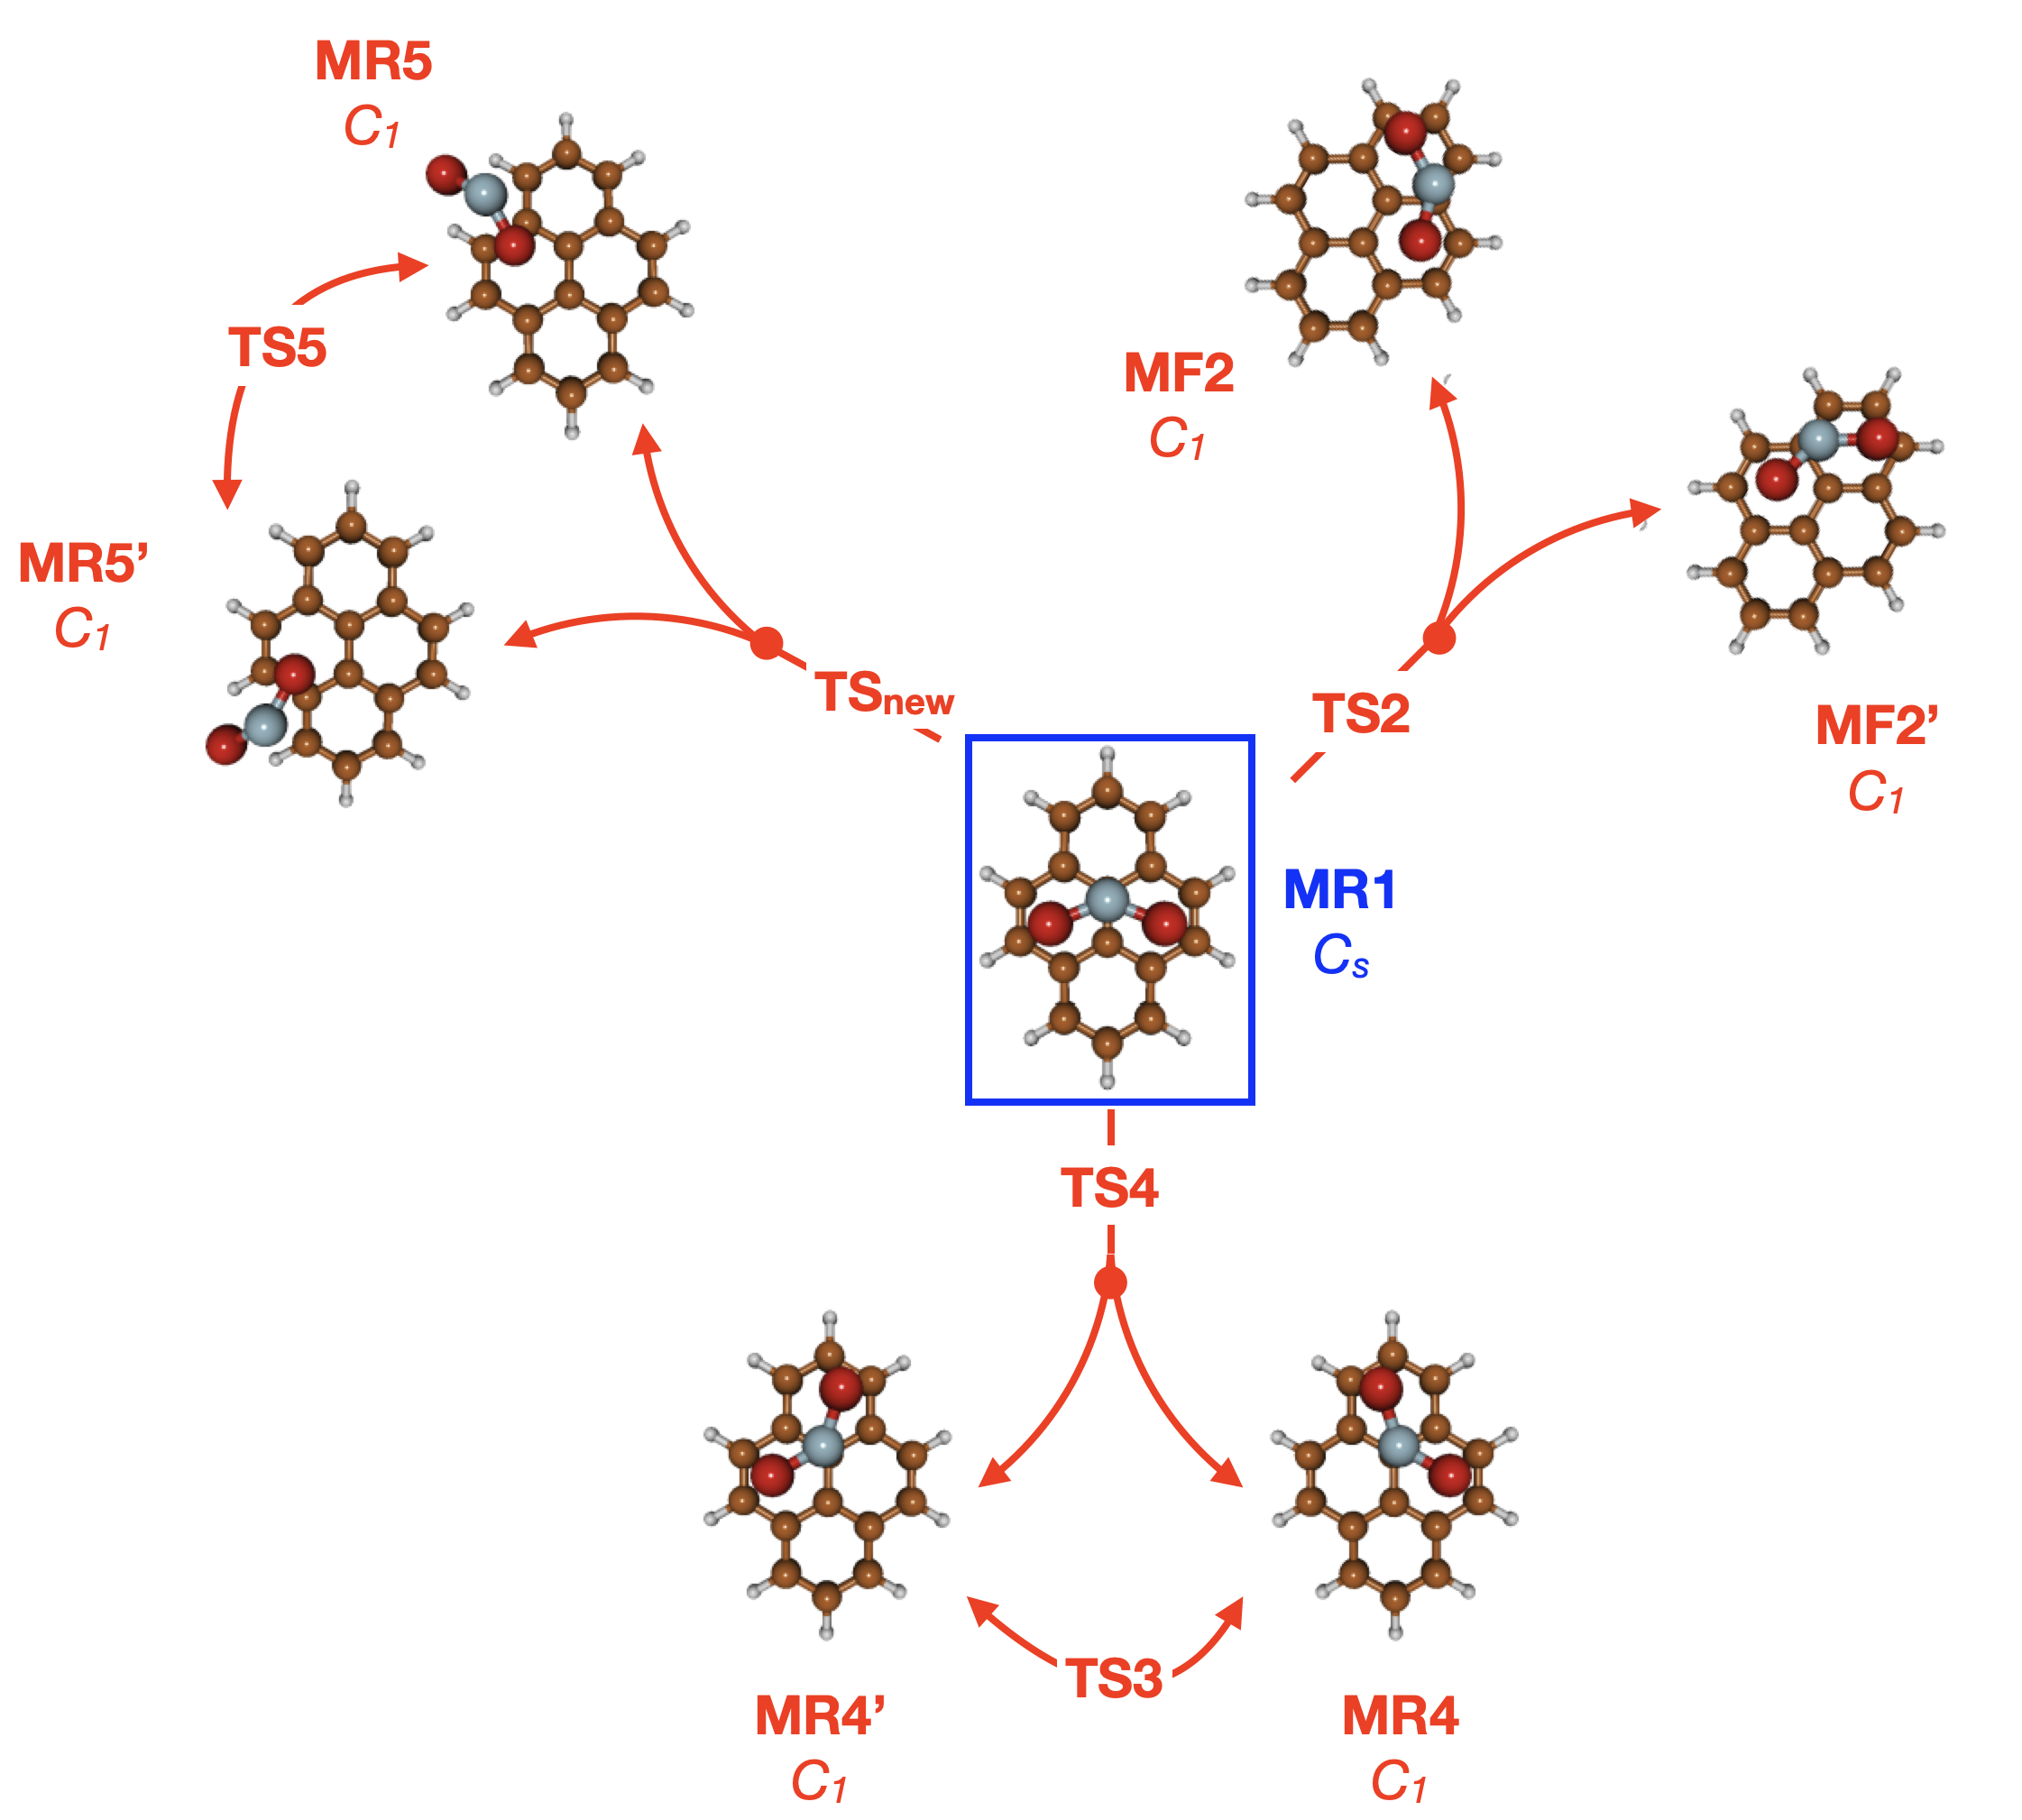
\includegraphics[scale=0.35]{pictures/pyrno2_rxn2.png}
%\end{center}
%
%The gathered topographical information has been used to obtain a global description (fit) of the interaction potential, necessary for the dynamical elucidation of the intermolecular interaction (physisorption), spectroscopic properties, and reactivity of the adsorbed species. To achieve this last goal, we have developed two different methodologies together with the corresponding software packages. The first one of them is the Specific Reaction Parameter Multigrid POTFIT (SRP-MGPF) algorithm, which is implemented in the SRPTucker package~\cite{panades2019specific}. This method computes chemically accurate (intermolecular) PESs through the reparametrization of semiempirical methods, which are subsequently tensor decomposed into Tucker form using MGPF~\cite{pel13:014108}. This software has been successfully interfaced with the Heidelberg version of the Multi-Configuration Time-Dependent Hartree (MCTDH) package~\cite{wor00:v81}. The second method allows for obtaining the PES directly in the mathematical form required by MCTDH, thence its name Sum-Of-Products Finite-Basis-Representation (SOP-FBR)~\cite{panades2020sop}. SOP-FBR constitutes an alternative approach to Neural Networks (NN)-fitting methods. The idea behind it is simple: from the basis of a low-rank Tucker expansion on the grid, we replace the grid-based basis functions by an expansion in terms of orthogonal polynomials. As in the previous method, smooth integration with MCTDH has been ensured. Both methods have been successfully benchmarked with a number of reference problems, namely: the Hénon-Heiles Hamiltonian, a global H\(_2\)O PES, and the HONO isomerization PES (6D). \\
%
%With the aid of all the above mentioned methods, we have tackled the computation of the global PES of the Pyrene-NO\(_2\) system. Suitable coordinate transformation routines have been developed to map the Cartesian coordinates to internal coordinates. In the physisorption domain, the evidence collected with vdW-TSSCDS has suggested that the geometry of the NO\(_2\) molecule is almost not perturbed in the stationary points with respect to the isolated molecule. This fact has enabled its treatment in a rigid monomer fashion (6D). The PESs will be used to obtain the electronic ground state (GS) and corresponding Zero-Point Energy (ZPE) of the system  with MCTDH\@. The ZPE can offer an accurate estimate of the adsorption energy of the NO\(_2\) molecule over the Pyrene. Additionally, the electronic absorption spectrum of the system will be obtained by computing the sum (weighted by the GS distribution) of the individual vertical excitations of each stationary point.\\
%
%\bibliographystyle{unsrt}
%\bibliography{Bibliography}

%----------------------------------------------------------------------------------------

\end{document}
